\chapter{Avaliação dos resultados do experimento}
	A entrada formada por ( b, a, f, m, s) é correspondido respectivamente pelas entradas
	SW[4], SW[3], SW[2], SW[1] e SW[0]. Para o estado Abrindo acende o \ac{led} verde (LEDG[0]) e
	para o estado de Fechando acende o \ac{led} vermelho (LEDR[0]). Assim, ao executar o
	\textit{test bench} obteve-se os resultados conforme as
	\autoref{figura:testBenchWaveMaquina} e \autoref{figura:testBenchTranscriptMaquina}.

	\begin{figure}[H]
		 \centering
		 \caption{\label{figura:testBenchWaveMaquina}\textit{Test bench Wave} do código da máquina.}
		 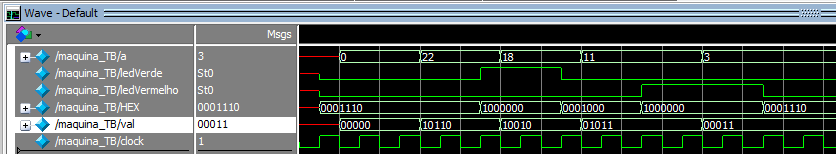
\includegraphics[width=1\textwidth]{img/maquina/testBenchWave}
	\end{figure}

	\begin{figure}[H]
		 \centering
		 \caption{\label{figura:testBenchTranscriptMaquina}\textit{Test bench Transcript} do código da máquina.}
		 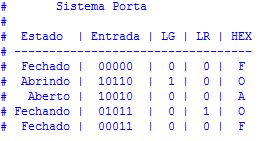
\includegraphics[width=0.5\textwidth]{img/maquina/testBenchTranscript}
	\end{figure}

	Como resultado do \textit{deploy} na placa, obteve o resultado confome as
	\autoref{figura:deployMaquina1}, \autoref{figura:deployMaquina2}, \autoref{figura:deployMaquina3},
	\autoref{figura:deployMaquina4}, \autoref{figura:deployMaquina5}, \autoref{figura:deployMaquina6} e
	\autoref{figura:deployMaquina7}.

		\begin{figure}[H]
			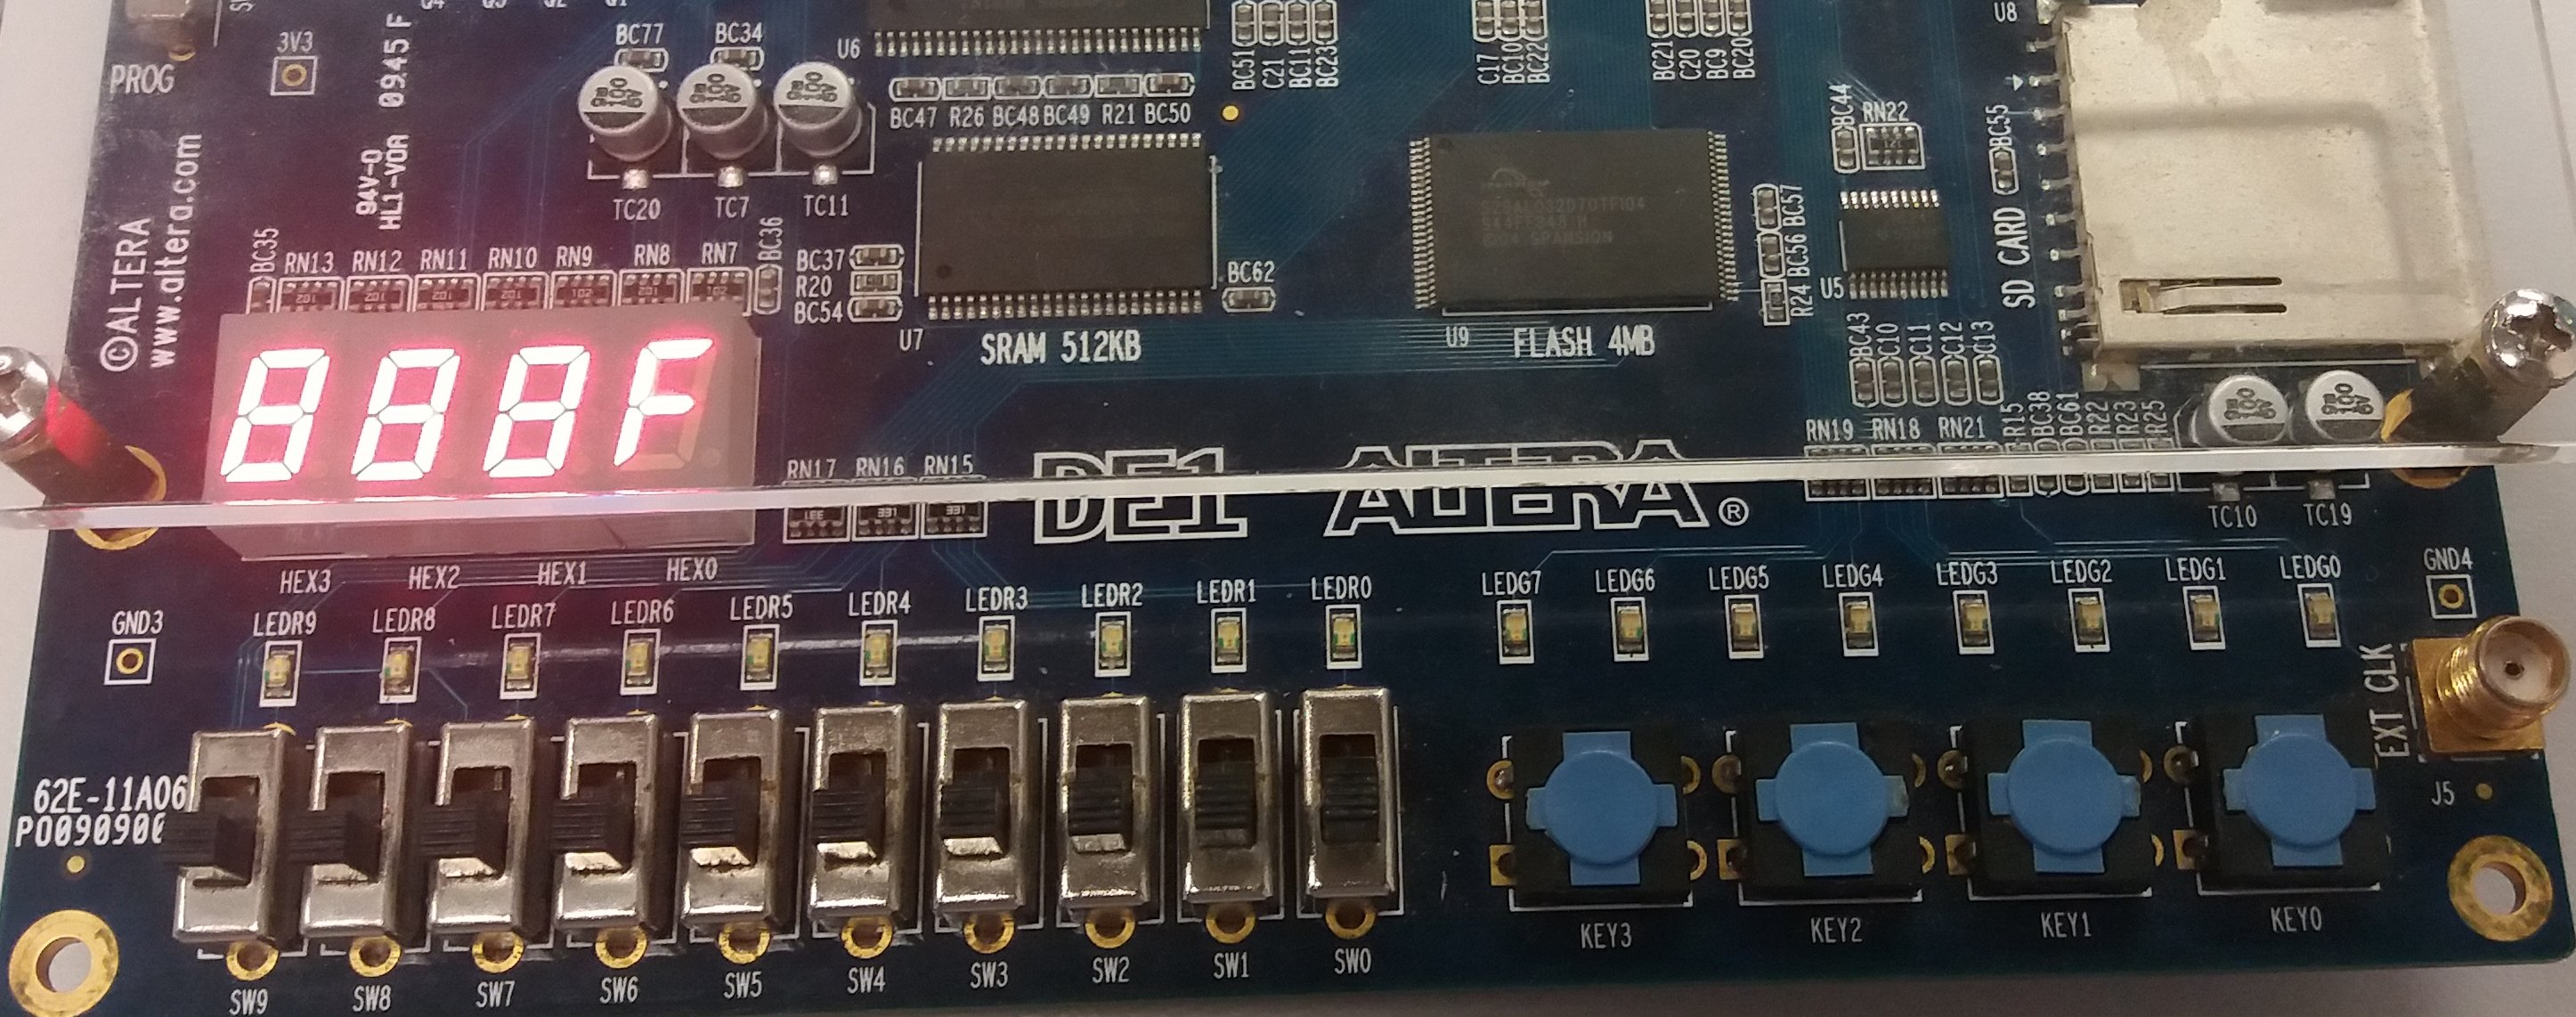
\includegraphics[width=1\textwidth]{img/maquina/placa/Fechado}
			\caption{Máquina no estado inicial (Fechado).\label{figura:deployMaquina1}}
		\end{figure}

		\begin{figure}[H]
			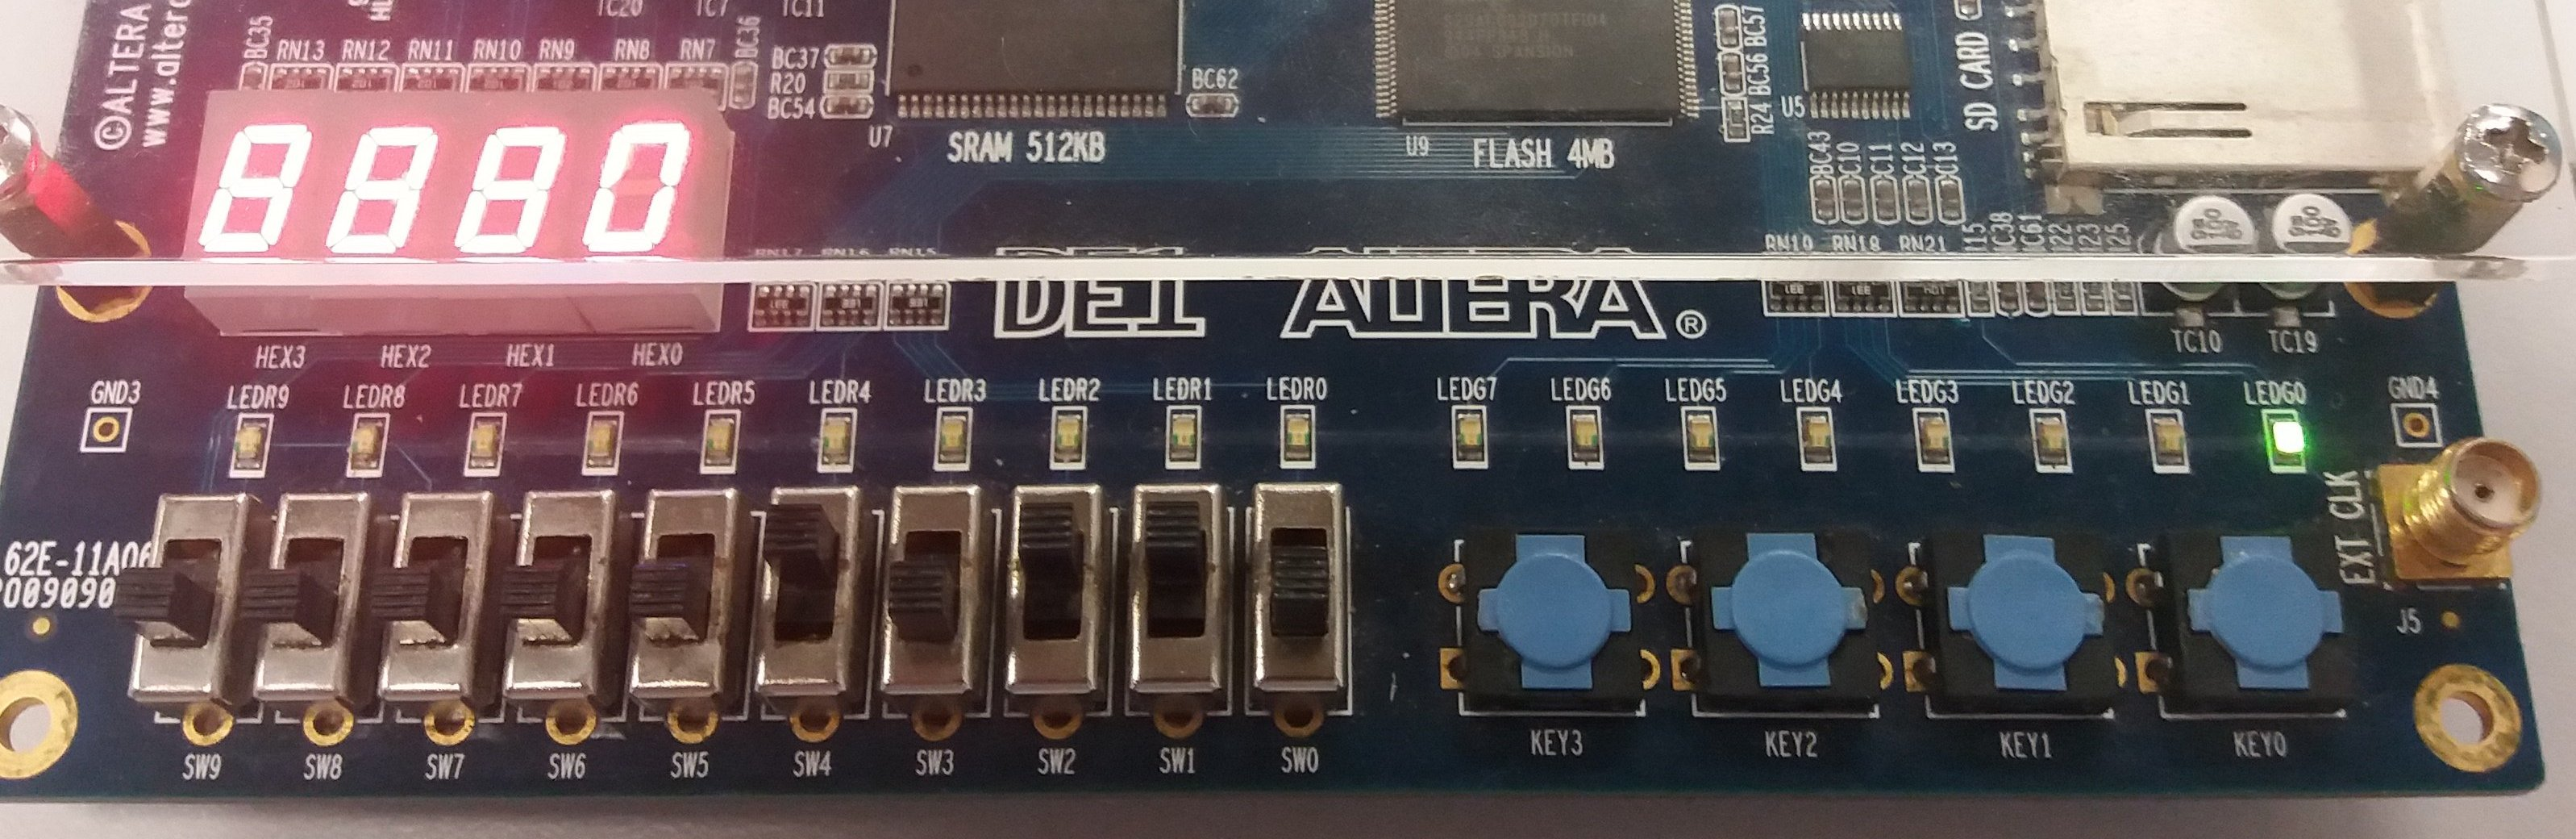
\includegraphics[width=1\textwidth]{img/maquina/placa/Fechado-Abrindo}
			\caption{Transição do estado Fechado para o Abrindo.\label{figura:deployMaquina2}}
		\end{figure}

		\begin{figure}[H]
			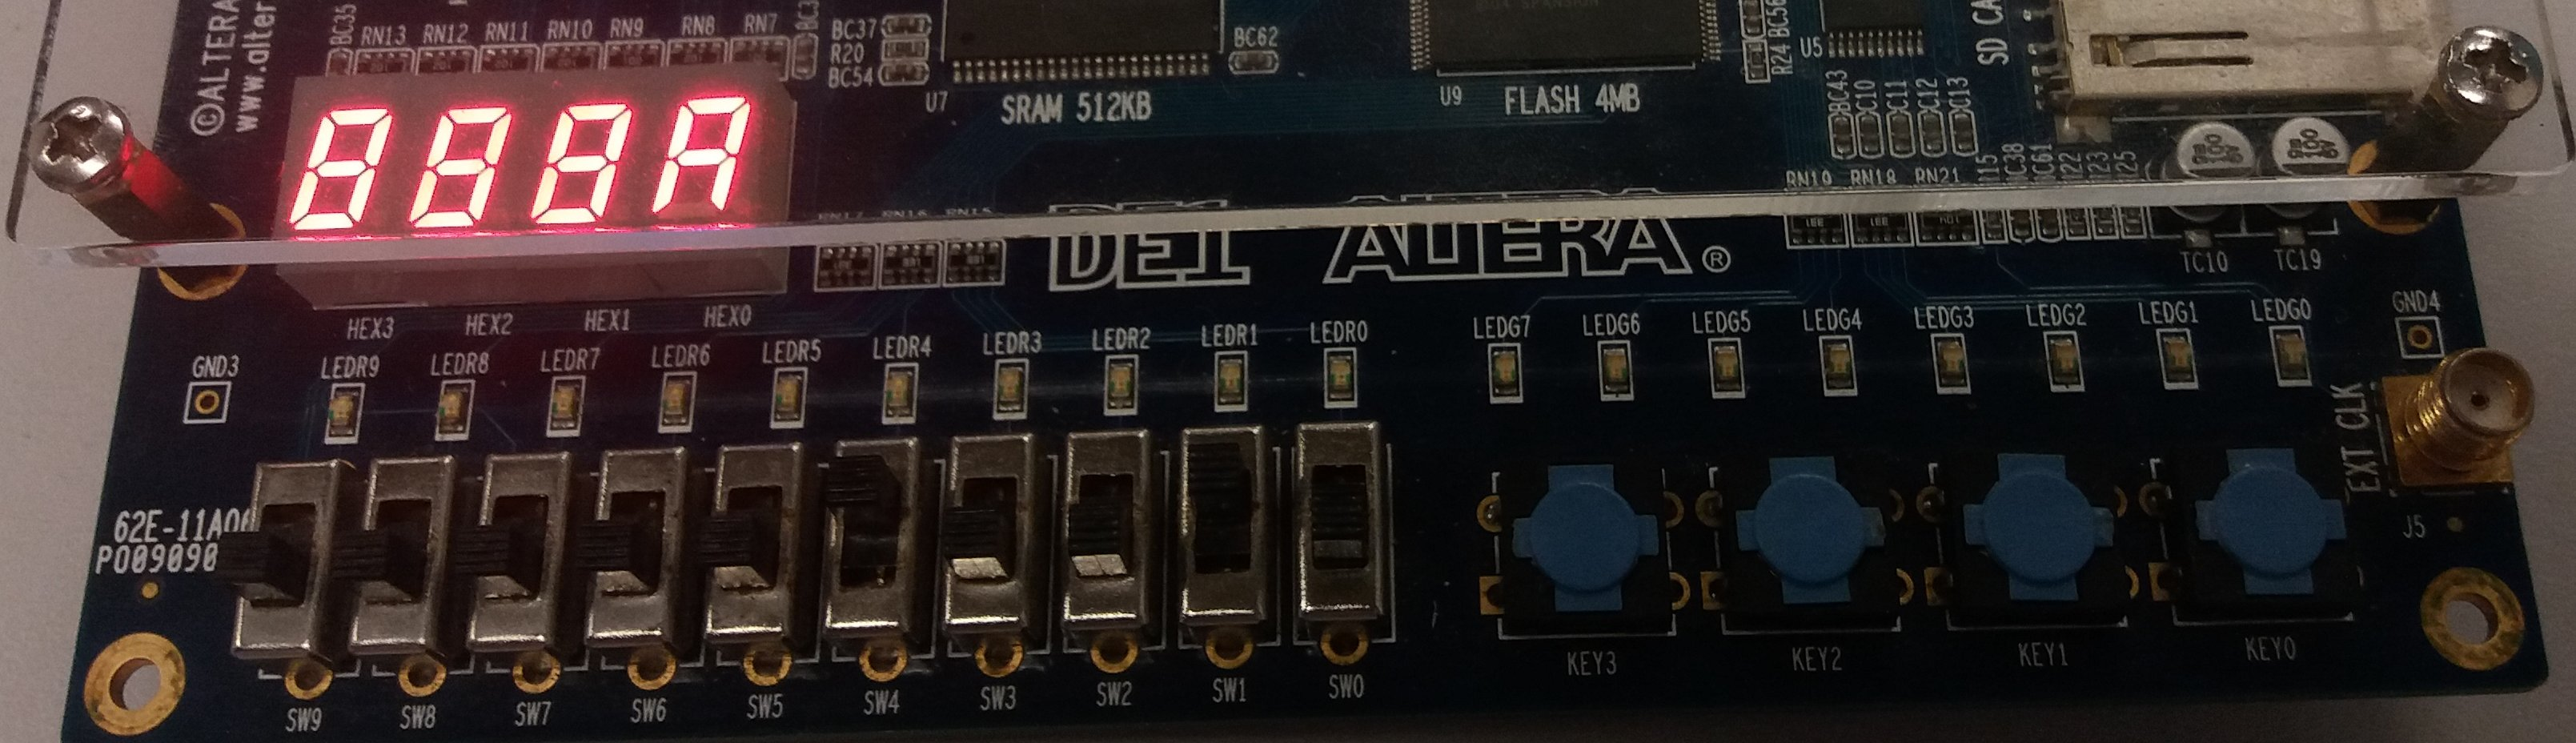
\includegraphics[width=1\textwidth]{img/maquina/placa/Abrindo-Aberto}
			\caption{Transição do estado Abrindo para o Aberto.\label{figura:deployMaquina3}}
		\end{figure}

		\begin{figure}[H]
			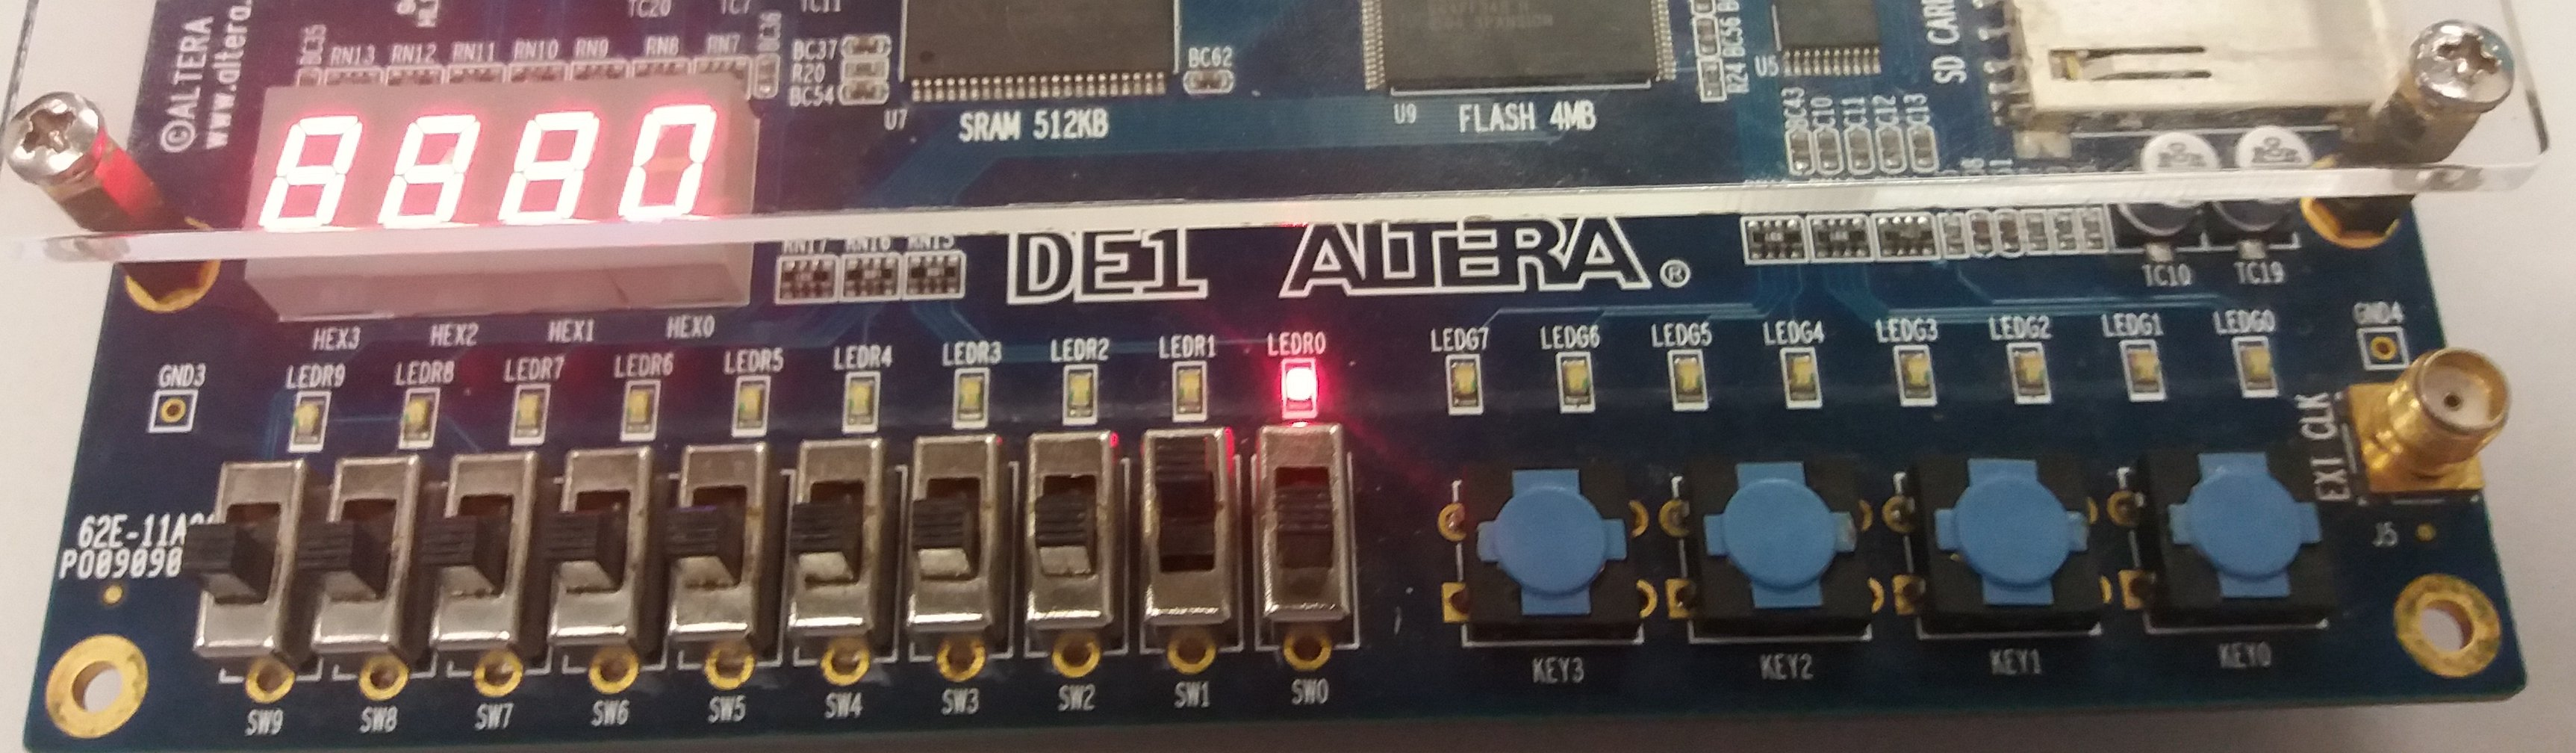
\includegraphics[width=1\textwidth]{img/maquina/placa/Abrindo-Fechando}
			\caption{Transição do estado Abrindo para o Fechando.\label{figura:deployMaquina4}}
		\end{figure}

		\begin{figure}[H]
			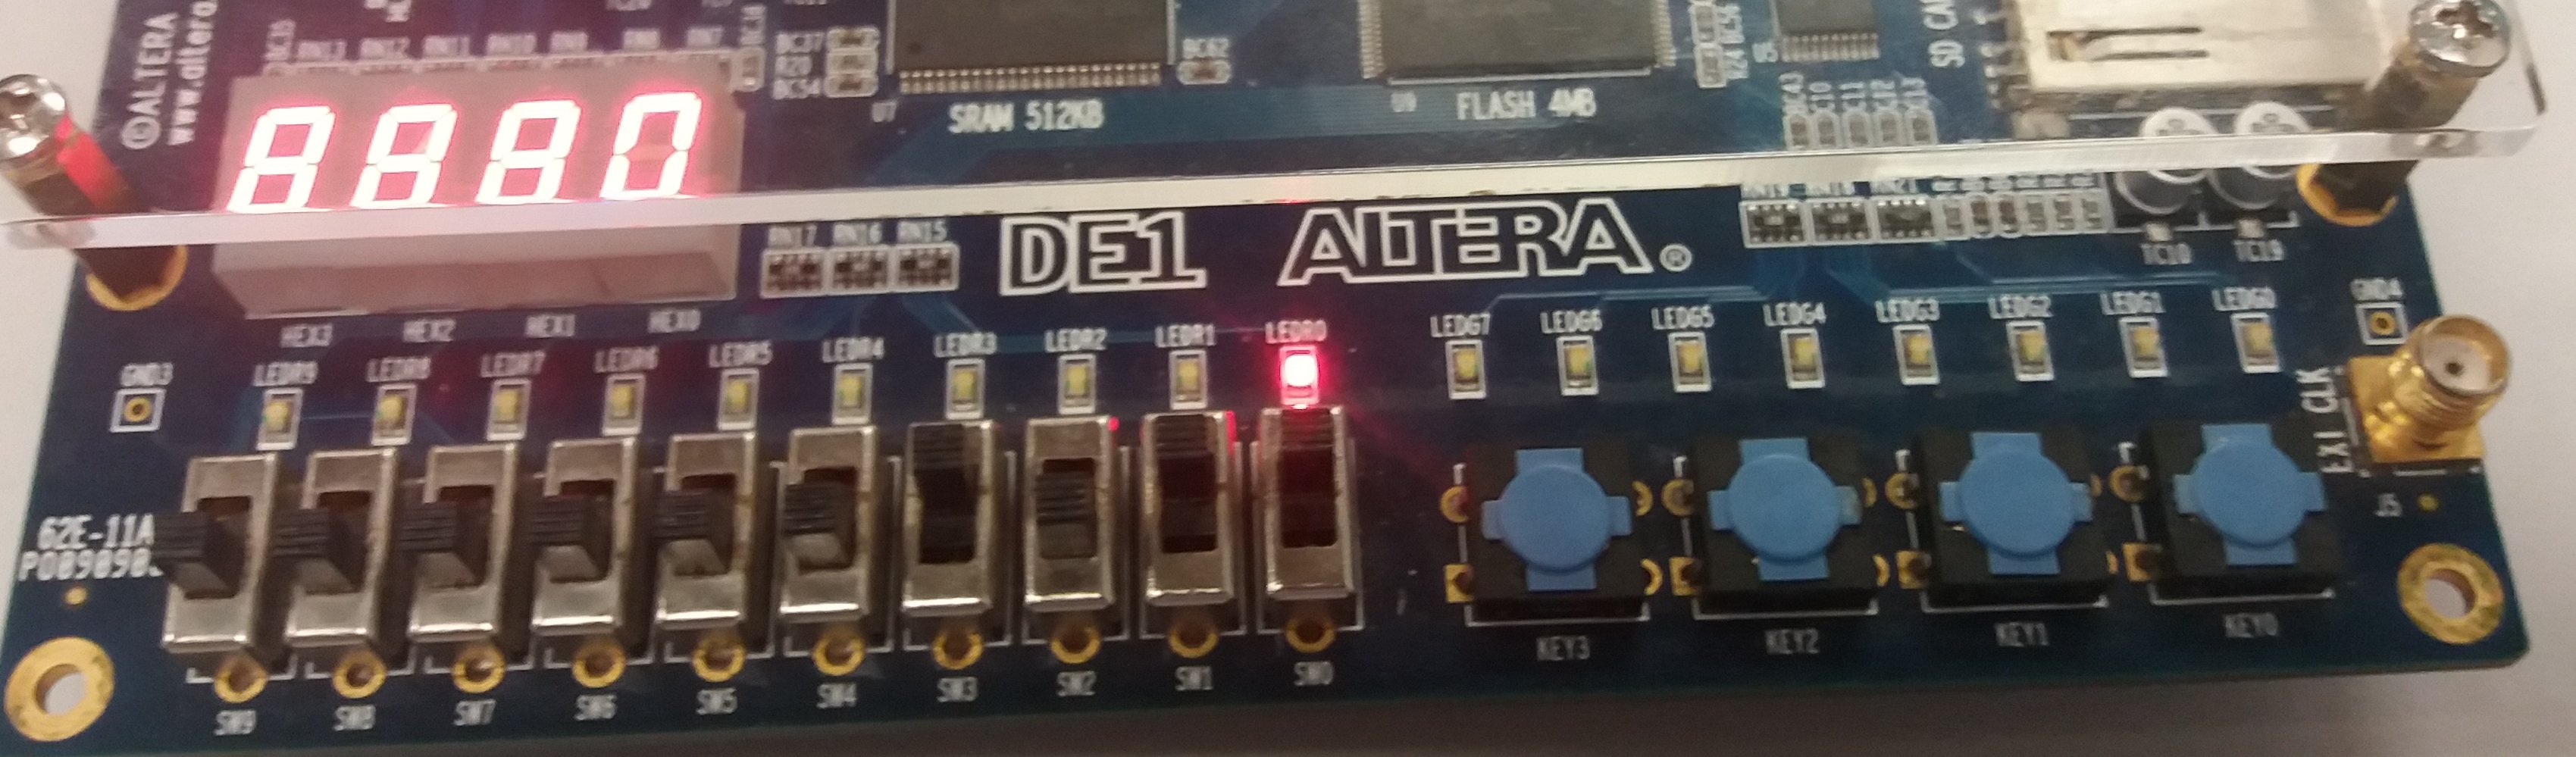
\includegraphics[width=1\textwidth]{img/maquina/placa/Aberto-Fechando}
			\caption{Transição do estado Aberto para o Fechando.\label{figura:deployMaquina5}}
		\end{figure}

		\begin{figure}[H]
			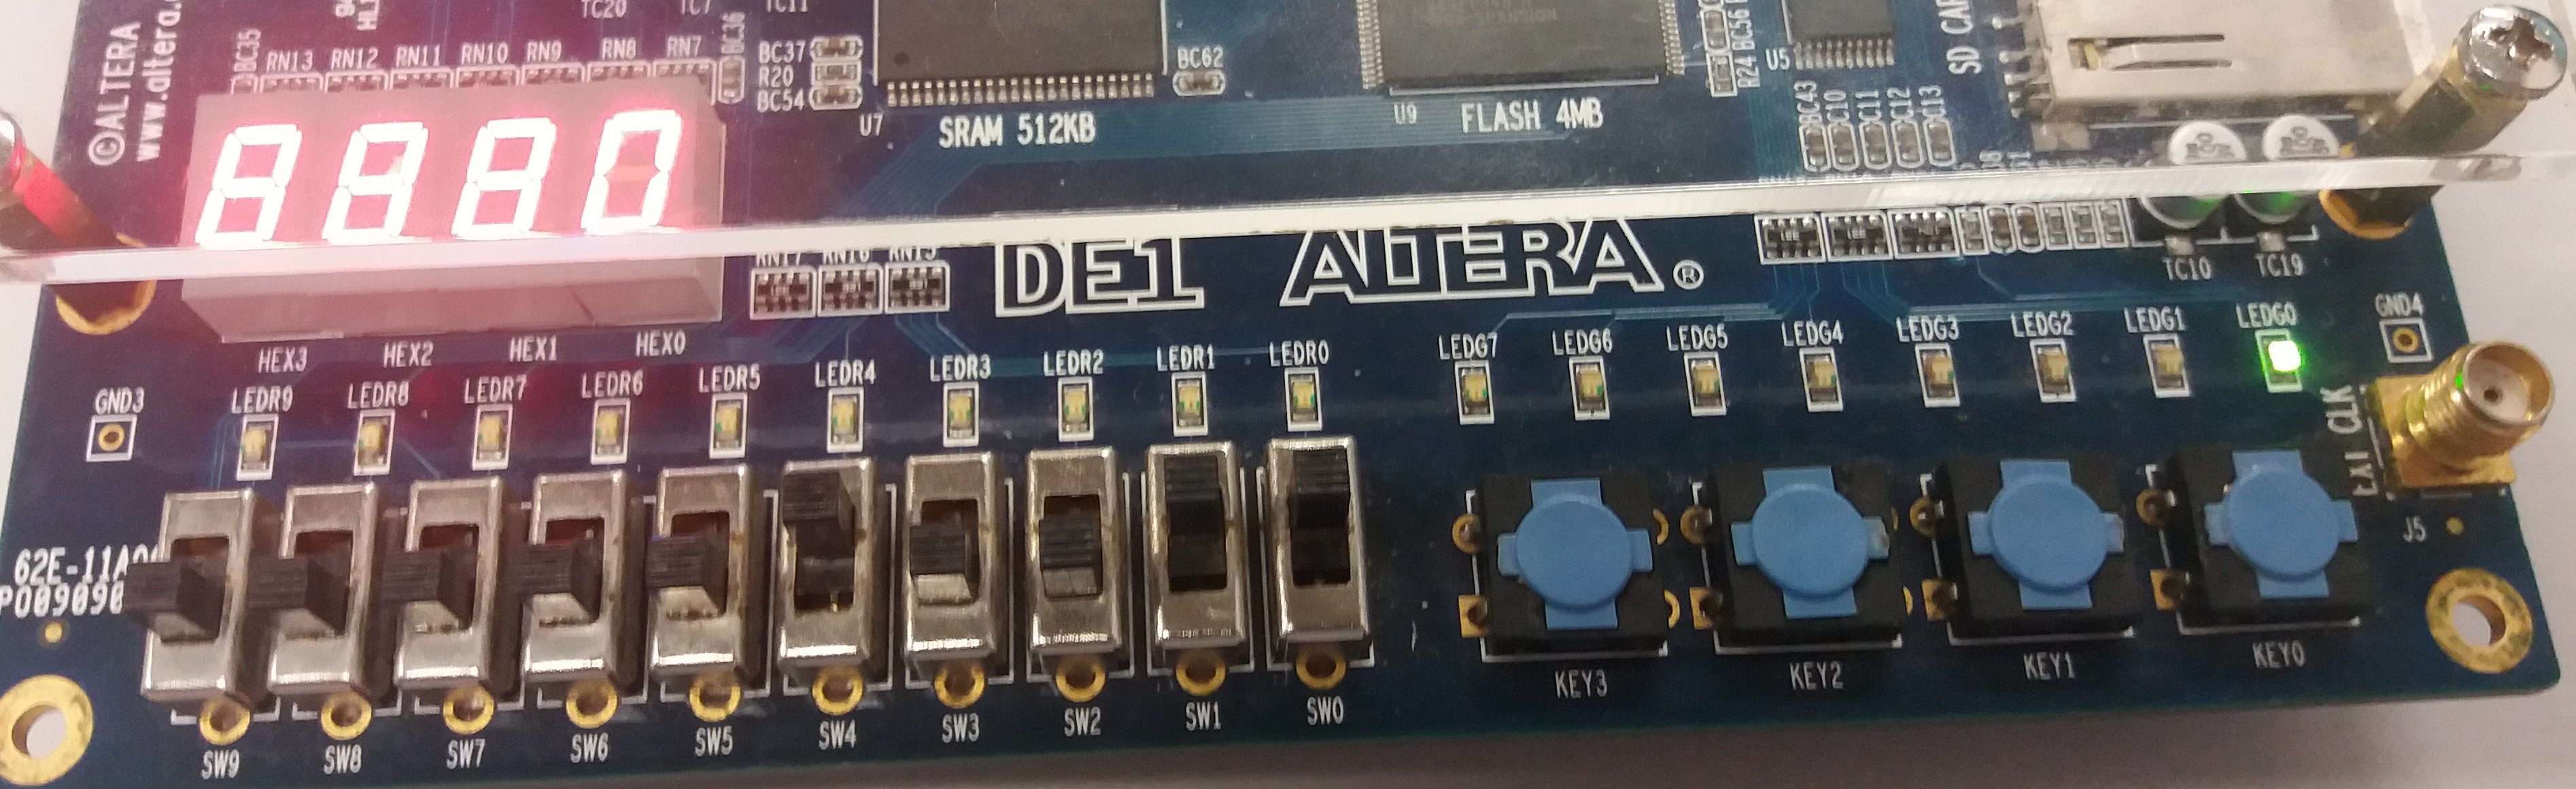
\includegraphics[width=1\textwidth]{img/maquina/placa/Fechando-Abrindo}
			\caption{Transição do estado Fechando para Abrindo.\label{figura:deployMaquina6}}
		\end{figure}

		\begin{figure}[H]
			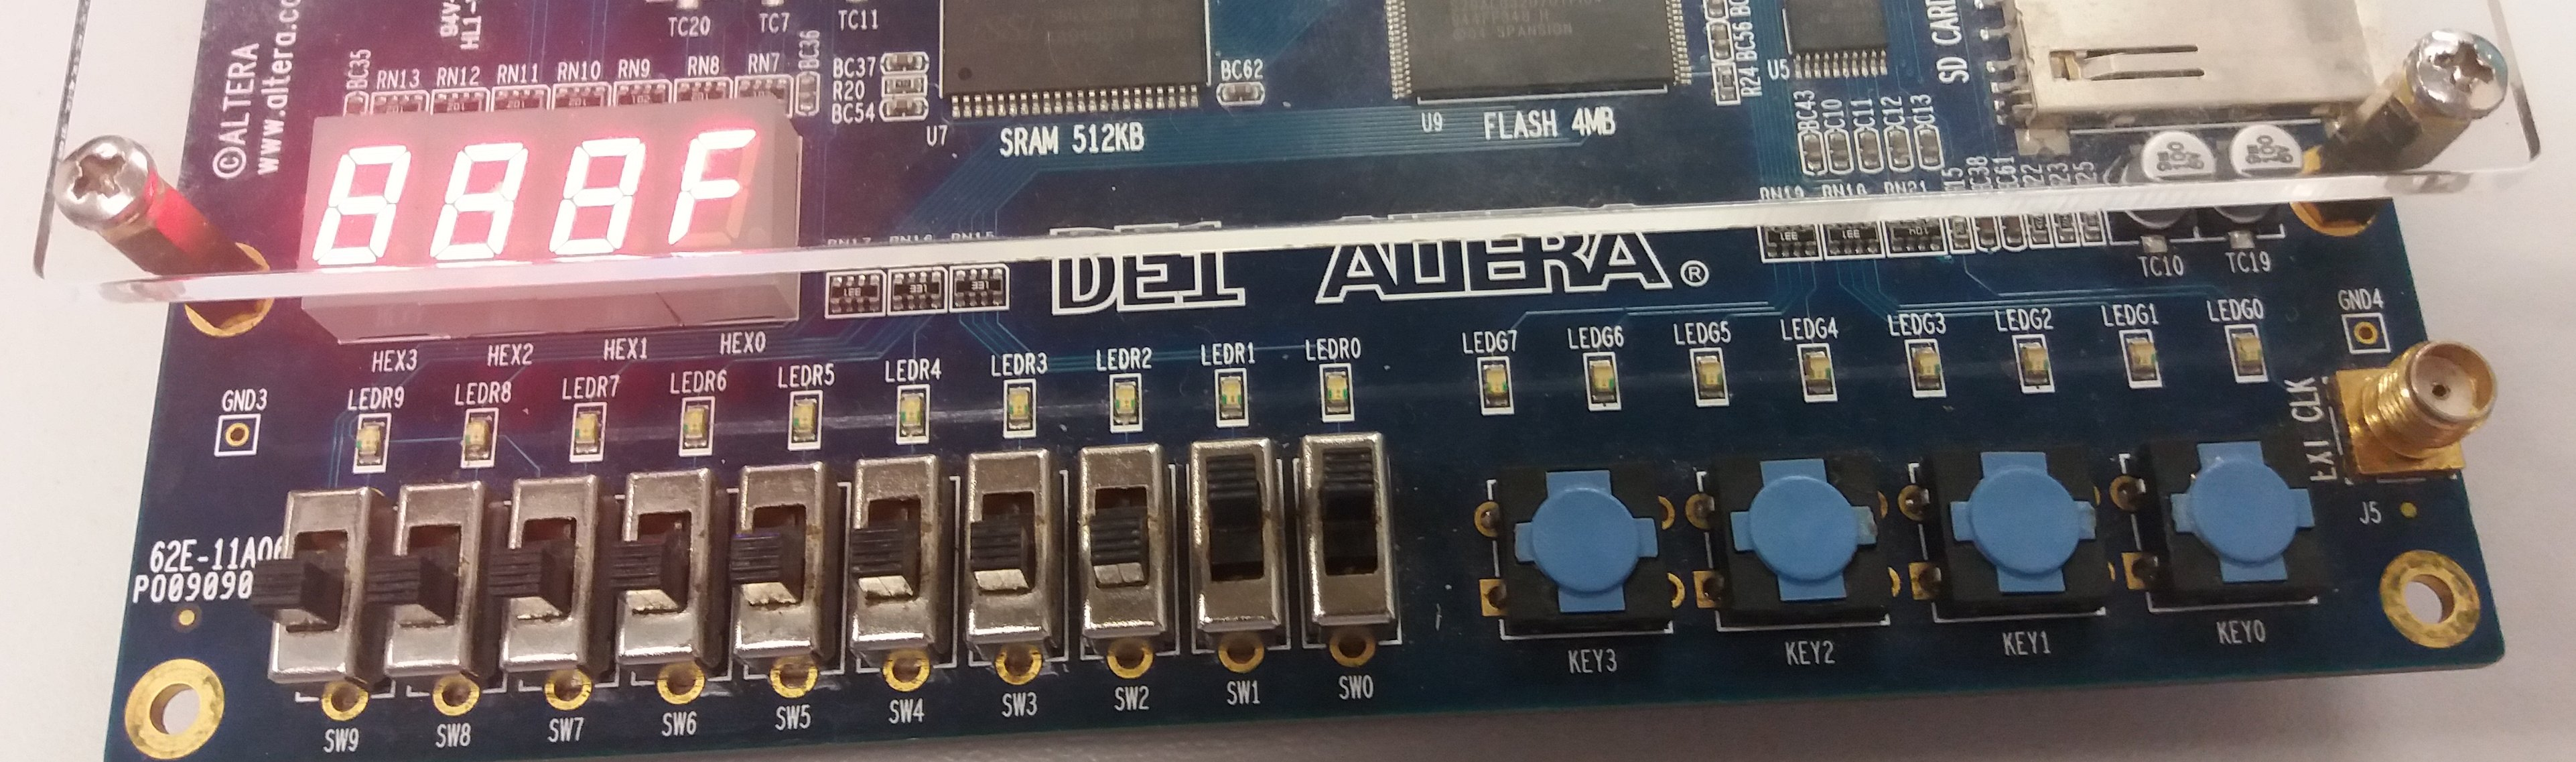
\includegraphics[width=1\textwidth]{img/maquina/placa/Fechando-Fechado}
			\caption{Transição do estado Fechando para Fechado.\label{figura:deployMaquina7}}
		\end{figure}


%Apresentar os resultados da simulação em software e da utilização do Kit DE1 e/ou
%protoboard. Utilizar figuras, descrevê-las e discuti-las.
